%\documentclass[letterpaper,draft]{beamer}
%\documentclass[letterpaper,handout]{beamer}
\documentclass[letterpaper, mathserif]{beamer}

%---multiple pages on one sheet, ADD for handout--
%\usepackage{pgfpages}
%\pgfpagesuselayout{4 on 1}[letterpaper, landscape, border shrink=1mm]
%-------------------------------------------------
\usepackage{amsmath,amsfonts}
%\usepackage[misc]{ifsym} % for the dice symbol \Cube{}
%\usepackage{booktabs}
%\usepackage{mdwlist}
%\usetheme{Copenhagen}
%\usetheme{warsaw}
\setbeamertemplate{navigation symbols}{}
\usepackage[english]{babel}
\def\ul{\underline}
% or whatever

\usepackage[latin1]{inputenc}
\subject{Talks}

\def\p{\mathrm P}
\def\E{\mathsf E}
\def\V{\mathsf{Var}}
\def\Sum{\sum\nolimits}
\def\Prod{\prod\nolimits}
\def\typo#1{\alert{#1}}
%-------------Answers------------
\def\Hide#1#2{\ul{~~~\onslide<#1>{\alert{#2}}~~~}}
\def\hide#1#2{\ul{~~\onslide<#1>{\alert{#2}}~~}}
%------Centered Page Number------
\defbeamertemplate{footline}{centered page number}
{%
  \hspace*{\fill}%
  %\usebeamercolor[fg]{page number in head/foot}%
  %\usebeamerfont{page number in head/foot}%
  \small Lecture \chapnum\ - \insertframenumber%
  \hspace*{\fill}\vskip2pt%
}

%\usepackage{tikz}
%\usebackgroundtemplate{%
%\tikz\node[opacity=0.3] {\includegraphics[height=\paperheight,widht=\paperwidth]{ctanlion}};}

%\usebackgroundtemplate{%
%  %\rule{0pt}{\paperheight}%
%  \parbox[c][\paperheight][c]{\paperwidth}{\centering\includegraphics[width=.65\paperwidth]{UClogo.pdf}}
%  %\hspace*{\paperwidth}
%}

\def\chapnum{8}
%--------------------------------
\setbeamertemplate{footline}[centered page number]

\title{STAT253/317 Winter 2017 Lecture \chapnum}
\date{}
\author{Yibi Huang}
\begin{document}
% ----------------------------------------------------------------------
%\begin{frame}\maketitle\begin{center}Generating Functions\end{center}
%\end{frame}
% ----------------------------------------------------------------------
\begin{frame}{STAT253/317 Lecture \chapnum ~ Generating Functions}
For a non-negative integer-valued random variable $T$, the generating function of $T$ is the expected value of $s^T$
as a function of $s$
\[
G(s)=\E[s^T]=\Sum_{k=0}^\infty s^k\p(T=k),
\]
in which $s^T$ is defined as 0 if $T=\infty$.

Since $0\le \p(T=k)\le 1$, the generating function is always well-defined for $-1\le s \le 1$
\end{frame}
% ----------------------------------------------------------------------
\begin{frame}{Examples of Generating Functions}
\begin{itemize}
\item If $T$ has a geometric distribution: $P(T=k)=p(1-p)^k$, $k=0,1,2,\ldots$,
the generating function of $T$ is
\[
G(s)=\Sum_{k=0}^\infty s^k\p(T=k)=\Sum_{k=0}^\infty s^kp(1-p)^k=\frac{p}{1-(1-p)s}
\]
\item If $T$ has a Binomial distribution $P(T=k)={n\choose k}p^k(1-p)^{n-k}$, $k=0,1,2,\ldots,n$,
the generating function of $T$ is
\begin{align*}
G(s)=\Sum_{k=0}^\infty s^k\p(T=k)
&=\Sum_{k=0}^\infty s^k{n\choose k}p^k(1-p)^{n-k}\\
&=(ps+(1-p))^n
\end{align*}
\end{itemize}
\end{frame}
% ----------------------------------------------------------------------
\begin{frame}{Properties of Generating Function}
\[
G(s)=\E[s^T]=\sum_{k=0}^\infty s^k\p(T=k)
\]

\begin{itemize}\itemsep=12pt
\item $G(s)$ is a power series converging absolutely for all $-1\!\le\!s\!\le\!1$.
since $0\le \p(T=k)\le 1$ and $\sum_k \p(T=k)\le 1.$
\item $\displaystyle G(1)=\p(T<\infty)
\begin{cases}
=1 & \text{if $T$ is finite w/ prob. 1}\\
<1 & \text{otherwise}
\end{cases}$
\item $P(T=k)=\dfrac{G^{(k)}(0)}{k!}$\par\medskip
Knowing $G(s)\Leftrightarrow$ Knowing $\p(T=k)$ for all $k=0,1,2,\ldots$
\end{itemize}
\end{frame}
% ----------------------------------------------------------------------
\begin{frame}{More Properties of Generating Functions}
\[
G(s)=\E[s^T]=\sum_{k=0}^\infty s^k\p(T=k)
\]
\begin{itemize}
\item $\E[T]=\lim_{s\to1^-} G'(s)$ if it exists because
$$G'(s)=\frac{d}{ds}\E[s^T]=\E[Ts^{T-1}]=\sum_{k=1}^\infty s^{k-1}k\p(T=k).$$

\item $\E[T(T-1)]=\lim_{s\to1^-} G''(s)$ if it exists because
$$G''(s)=\E[T(T-1)s^{T-2}]=\Sum_{k=2}^\infty s^{k-2}k(k-1)\p(T=k)$$
\item If $T$ and $U$ are \textbf{independent}  non-negative-integer-valued random variables, with generating function $G_T(s)$ and $G_U(s)$ respectively, then the generating function of $T+U$ is
    $$G_{T+U}(s)=\E[s^{T+U}]=\E[s^{T}]\E[s^{U}]=G_T(s)G_U(s)$$
\end{itemize}
\end{frame}
% ----------------------------------------------------------------------
% ----------------------------------------------------------------------
%\begin{frame}{Mean of $N_{0,n}$}
%Recall that $N_{0n}=N_{01}+N_{12}+\ldots+N_{n-1,n}$
%\begin{align*}
%\E[N_{0n}]&=m_{0}+m_{1}+\ldots+m_{n-1}\\
%&=\begin{cases}
%\frac{n}{p-q}-\frac{2pq}{(p-q)^2}[1-(\frac{q}{p})^n] &\text{if } p\neq 0.5\\
%n^2 & \text{if } p= 0.5
%\end{cases}
%\end{align*}
%When
%$$
%\begin{array}{cll}
%p>0.5& \E[N_{0n}]\approx \frac{n}{p-q}-\frac{2pq}{(p-q)^2} & \text{linear in }n\\[5pt]
%p=0.5& \E[N_{0n}]= n^2 & \text{quadratic in }n\\[5pt]
%p<0.5& \E[N_{0n}]=O(\frac{2pq}{(p-q)^2}(\frac{q}{p})^n) & \text{exponential in }n
%\end{array}
%$$
%\end{frame}
% ----------------------------------------------------------------------
%\begin{frame}{Example: Symmetric Random Walk on $(-\infty,\infty)$}
%State space $=\{\ldots,-2,-1,0,1,2,\ldots\}$
%$$
%P_{i,i+1}=P_{i,i-1}=1/2,\quad \text{for all integer } i
%$$\vspace{-10pt}
%\begin{itemize}
%\item 1 classes, recurrent, null-recurrent or positive-recurrent?
%\item For $i,j$, define $N_{ij}=\min\{m> 0: X_m=j|X_0=i\}$.
%\item Note $N_{00}=1+N_{10}$
%\item Given $X_0=1$
%\begin{equation}\label{eq:T2TT}
%N_{10}=
%\begin{cases}
%1 & \text{if } X_1=0\\
%1 + N_{21}+ N_{10}' &\text{if } X_1=2
%\end{cases}
%\end{equation}
%Note $N_{21}$ and $N_{10}'$ are independent and have the same distribution as $N_{10}$ (Why?)
%\end{itemize}
%\end{frame}
% ----------------------------------------------------------------------
%\begin{frame}{Generating Function of $N_{10}$}
%Let $G(s)$ be the generating function of $N_{10}$.
% From \eqref{eq:T2TT}, we know that
%$$
%G(s)=\frac{1}{2}s+\frac{1}{2} \E[s^{1 + N_{21}+ N_{10}'}]=\frac{1}{2}s+\frac{1}{2}sG(s)^2
%$$
%which is a quadratic equation in $G(s)$. The two roots are
%$$
%G(s)=\frac{1\pm\sqrt{1-s^2}}{s}
%$$
%Since $G(s)$ must lie between 0 and 1 when $0<s<1$. So
%$$
%G(s)=\frac{1-\sqrt{1-s^2}}{s}
%$$
%Note that $$G'(s)=\frac{1}{\sqrt{1-s^2}+1-s^2},\quad \E[N_{10}]=\lim_{s\to 1^-}G'(s)=\infty$$
%which implies $\E[N_{00}]=1+\E[N_{10}]=\infty$.\\
%$\Rightarrow$ Symmetric random walk is null recurrent.
%\end{frame}
%% ----------------------------------------------------------------------
%\begin{frame}
%The power series expansion of $G(s)=\frac{1-\sqrt{1-s^2}}{s}$ can be found via Newton's binomial formula
%$$(1-s^2)^{\alpha}=\sum_{k=0}^{\infty}{\alpha \choose k}(-s^2)^k$$
%where ${\alpha \choose 0}=1$ and for $k\ge 1$, ${\alpha \choose k}=\prod_{i=0}^{k-1}(\alpha-i)/k!.$
%\begin{align*}
%{1/2 \choose k}
%&=\frac{\frac{1}{2} (\frac{1}{2}-1)(\frac{1}{2}-2)(\frac{1}{2}-3)\ldots(\frac{1}{2}-k+1)}{k!}\\
%&=\frac{(-1)^{k-1}1\cdot 1\cdot 3\cdot 5\ldots(2k-3)}{2^k k!}\\
%&=\frac{(-1)^{k-1}1\cdot 1\cdot 3\cdot 5\ldots(2k-3)(2k-1)}{2^k k!(2k-1)}\\
%&=\frac{(-1)^{k-1}\frac{(2k-1)!}{2^{k-1}(k-1)!}}{2^k k!(2k-1)}
%=\frac{(-1)^{k-1}}{2^{2k-1}(2k-1)}{2k-1\choose k}
%\end{align*}
%\end{frame}
%% ----------------------------------------------------------------------
%\begin{frame}
%From all the above we have
%\begin{align*}
%G(s)&=\frac{1-\sum_{k=0}^{\infty}{1/2 \choose k}(-s^2)^{{k}}}{s}=-\sum_{k=1}^{\infty}(-1)^{k}{1/2 \choose %k}s^{2k-1}\\
%&=\sum_{k=1}^{\infty}\frac{1}{2^{2k-1}(2k-1)}{2k-1\choose k}s^{2k-1}
%\end{align*}
%So the distribution of $N_{10}$ is
%\begin{align*}
%\p(N_{10}=2k-1)&=\frac{1}{2^{2k-1}(2k-1)}{2k-1\choose k}\\
%\p(N_{10}=2k)  &= 0
%\end{align*}
%for $k=0,1,2,\ldots$
%\end{frame}
% ----------------------------------------------------------------------
\begin{frame}{4.7 Branching Processes Revisit}
Recall a Branching Process is a population of individuals in which
\begin{itemize}
\item all individuals have the same lifespan, and
\item each individual will produce a random number of offsprings at the end of its life
\end{itemize}
Let $X_n=$ size of the $n$th generation, $n=0,1,2,\ldots$.
Let $Z_{n,i}=\#$ of offsprings produced by the $i$th individuals in the $n$th generation. Then
\begin{equation}\label{eq:branching}
X_{n+1} =\Sum_{i=1}^{X_{n}}Z_{n,i}
\end{equation}
Suppose  $Z_{n,i}$'s are i.i.d with probability mass function
$$P(Z_{n,i}=j)=P_j,\; j \ge 0.$$
We suppose the non-trivial case that $P_j < 1$ for all $j \ge 0$.

$\{X_n\}$ is a Markov chain with state space $=\{0,1,2,\ldots\}$.
\end{frame}
% ----------------------------------------------------------------------
\begin{frame}{Generating Functions of the Branching Processes}
Let $g(s)=\E[s^{Z_{n,i}}]=\sum_{k=0}^{\infty}P_ks^k$ be the generating function of $Z_{n,i}$, and
$G_n(s)$ be the generating function of $X_n$, $n=0,1,2,\ldots$.
Then $\{G_n(s)\}$ satisfies the following two iterative equations.
\begin{align*}
\text{(i)}  &\; G_{n+1}(s)=G_n(g(s))\quad\text{for }n=0,1,2,\ldots\\
\text{(ii)} &\; G_{n+1}(s)=g(G_n(s))\quad\text{if $X_0=1$, for }n=0,1,2,\ldots
\end{align*}
{\em Proof of (i).}\vspace{-8pt}
\begin{align*}
\E[s^{X_{n+1}}|X_{n}]=\E\left[s^{\sum_{i=1}^{X_{n}}Z_{n,i}}\right]&=\E\Big[\Prod_{i=1}^{X_{n}}s^{Z_{n,i}}\Big]\\
&=\Prod_{i=1}^{X_{n}}\E[s^{Z_{n,i}}]&\text{by indep. of $Z_{n,i}$'s}\\
&=\Prod_{i=1}^{X_{n}}g(s)&\text{as }g(s)=\E[s^{Z_{n,i}}]\\
&=g(s)^{X_{n}}
\end{align*}
From which, we have
$$G_{n+1}(s)=\E[s^{X_{n+1}}]=\E[\E[s^{X_{n+1}}|X_n]]=\E[g(s)^{X_n}]=G_n(g(s))$$
since $G_n(s)=\E[s^{X_{n}}]$.

\end{frame}
% ----------------------------------------------------------------------
\begin{frame}{Proof of (ii) $G_{n+1}(s)=g(G_n(s))$ if $X_0=1$}\small
Suppose there are $k$ individuals in the first generation ($X_1=k$).
Let $Y_i$ be the number offspring of the $i$th individual in the first generation in the $(n+1)$st generation. Obviously,
$$X_{n+1}=Y_1+\ldots+Y_k.$$
Observe $Y_1,\ldots,Y_k$'s are indep and each has the same distn. as $X_n$ since they are all the size of the $n$th generation of a single ancestor. Thus, by indep. of $Y_i$'s
\[
\E[s^{X_{n+1}}|X_{1}=k]=\E\big[s^{Y_1+\ldots+Y_k}\big]=\E\left[\Prod_{i=1}^{k}s^{Y_i}\right]=\Prod_{i=1}^{k}\E[s^{Y_{i}}]
\]
Since $Y_i$'s have the same dist'n as $X_n$ and $G_n(s)=\E[s^{X_{n}}],$ we have
\[\E[s^{X_{n+1}}|X_{1}=k]=\Prod_{i=1}^{k}G_n(s)=(G_n(s))^{k}\]
Since $X_0=1$, $X_1=Z_{1,1}$, and hence $\p(X_1=k)=P_k$.
$$G_{n+1}(s)=\E[s^{X_{n+1}}]
=\sum_{k=0}^{\infty}\E[s^{X_{n+1}}|X_1=k]P_k=\sum_{k=0}^{\infty}(G_n(s))^k P_k=g(G_n(s)),$$
where the last equality comes from that $g(s)=\sum_{k=0}^{\infty}P_k s^k.$
\end{frame}
% ----------------------------------------------------------------------
\begin{frame}{Example: calculating distributions of $X_n$}
Suppose $X_0=1$, and $(P_0,P_1,P_2)=(1/4,1/2,1/4)$. Find the distribution of $X_2$.\par
{\em Sol.}
$$g(s)=\frac{1}{4}s^0+\frac{1}{2}s^1+\frac{1}{4}s^2=(1+s)^2/4.$$
Since $X_0=1$, $G_0(s)=\E[s^{X_0}]=\E[s^{1}]=s$. From (i) we have
\begin{align*}
G_1(s)&=G_0(g(s))=g(s)=(1+s)^2/4\\
G_2(s)&=G_1(g(s))=\frac{1}{4}(1+\frac{1}{4}(1+s)^2)^2
%=\frac{1}{4}(\frac{5}{4}+\frac{1}{2}s+\frac{1}{4}s^2)^2\\
      =\frac{1}{64}(5+2s+s^2)^2\\
      &=\frac{1}{64}(25+20s+14s^2+4s^3+s^4)
      %&=\frac{25}{64}+\frac{5}{16}s+\frac{7}{32}s^2+\frac{1}{16}s^2+\frac{1}{65}s^4
      =\sum_{k=0}^{\infty}\p(X_2=k)s^k
\end{align*}
The coefficient of $s^k$ in the polynomial of $G_2(s)$ is the chance that $X_2=k$.
\begin{center}\vspace{-10pt}
\renewcommand{\arraystretch}{1.25}
\begin{tabular}{c|ccccc}
$k$         & 0 & 1 & 2 & 3 & 4\\
\hline
$\p(X_2=k)$ &$\frac{25}{64}$&$\frac{20}{64}$&$\frac{14}{64}$&$\frac{4}{64}$&$\frac{1}{64}$
\end{tabular}
\end{center}
and $\p(X_2=k)=0$ for $k\ge 5.$
\end{frame}
% ----------------------------------------------------------------------
\begin{frame}{Extinction Probability of a Branching Process}
\begin{align*}
\text{Let }\pi_0 &= \lim_{n\to\infty}\p(X_n = 0|X_0 = 1)\\
      &=\p(\text{the population will eventually die out}|X_0 = 1)
\end{align*}
As $G_n(s)=\E[s^{X_n}]=\sum_{k=0}^{\infty}P(X_n=k)s^k$, plugging in $s=0$, we get
\[
G_n(0)=P(X_n=0)=P(\text{extinct by the $n$th generation}).
\]
Recall that if $X_0=1$, $G_1(s)=g(s)$, and $G_{n+1}(s)=g(G_n(s))$.
We can compute $G_n(0)$ iteratively as follows
\begin{align*}
G_1(0)&=g(0)\\
G_{n+1}(0)&=g(G_n(0)),\quad n=1,2,3,\ldots
\end{align*}
Finally, we can get the extinction probability by taking the limit
\[\pi_0=\lim_{n\to\infty}G_n(0).\]
\end{frame}
% ----------------------------------------------------------------------
\begin{frame}{Extinction Probability of a Branching Process}
If $X_0=1$, the extinction probability $\pi_0$ is a {\bf smallest root}
of the equation
\begin{equation}\label{eq:extinct}
g(s)=s
\end{equation}
in the range $0<s<1$,
where $g(s)=\sum_{k=0}^{\infty}P_ks^k$ is the generating function of $Z_{n,i}$.

{\em Proof.} 
\begin{center}
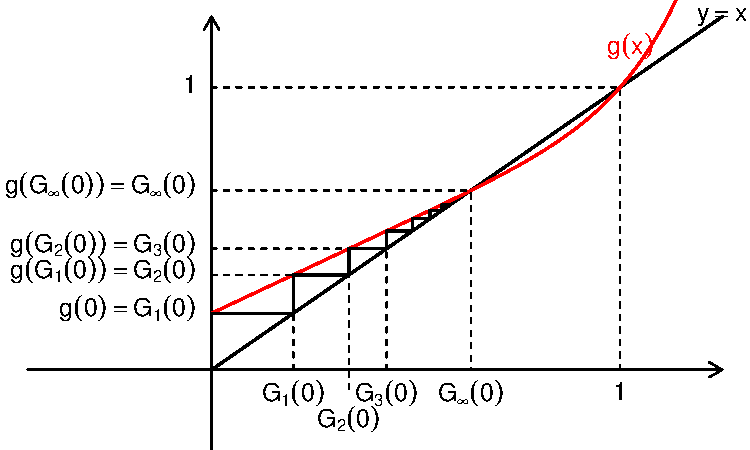
\includegraphics[width=0.85\textwidth]{extinction.pdf}
\end{center}
\end{frame}
% ----------------------------------------------------------------------
\begin{frame}{A Branching Process Will Become Extinct If $\mu\le 1$}
Let $\mu=\E[Z_{n,i}]=\Sum_{j=0}^{\infty}jP_j$. If $\mu\le 1$, the extinction probability $\pi_0$ is 1.

{\em Proof.}
\begin{center}
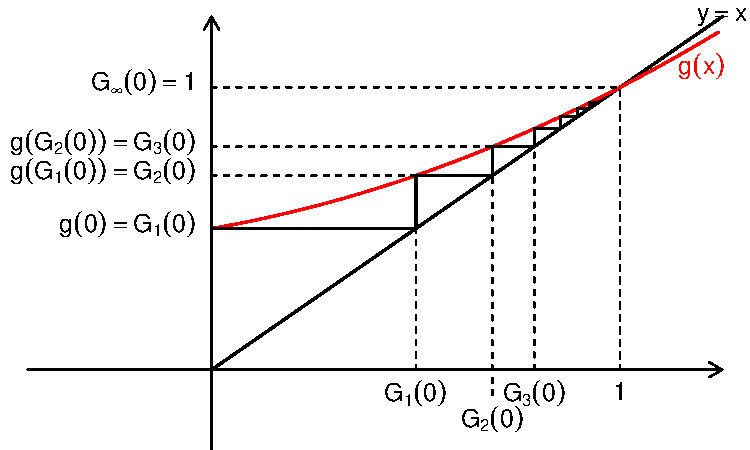
\includegraphics[width=\textwidth]{extinction2.pdf}
\end{center}
\end{frame}
% ----------------------------------------------------------------------
\begin{frame}{Formal Proof}
Let $h(s)=g(s)-s$. Since $g(1)=1$, $g'(1)=\mu$,
\begin{align*}
h(1)&=g(1)-1=0,\\
h'(s)&=\Big(\sum_{j=1}^{\infty}jP_js^{j-1}\Big)-1
   \le\Big(\sum_{j=1}^{\infty}jP_j\Big)-1=\mu-1 \quad\text{for }0\le s < 1
\end{align*}
\begin{align*}
\text{Thus }\mu\le 1
&\Rightarrow h'(s)\le0\text{ for }0\le s< 1\\
&\Rightarrow h(s)\text{ is non-increasing in }[0,1)\\
&\Rightarrow h(s)> h(1)=0\text{ for }0\le s < 1\\
&\Rightarrow g(s)>s&\text{ for }0\le s< 1\\
&\Rightarrow \text{ There is no root in [0,1)}.
\end{align*}
\end{frame}
% ----------------------------------------------------------------------
\begin{frame}{Extinction Probability When $\mu>1$}
If $\mu>1$, there is a unique root of the equation $g(s)=s$ in the domain $[0,1)$,
and that is the extinction probability.\par\medskip
{\em Proof.}

\begin{center}
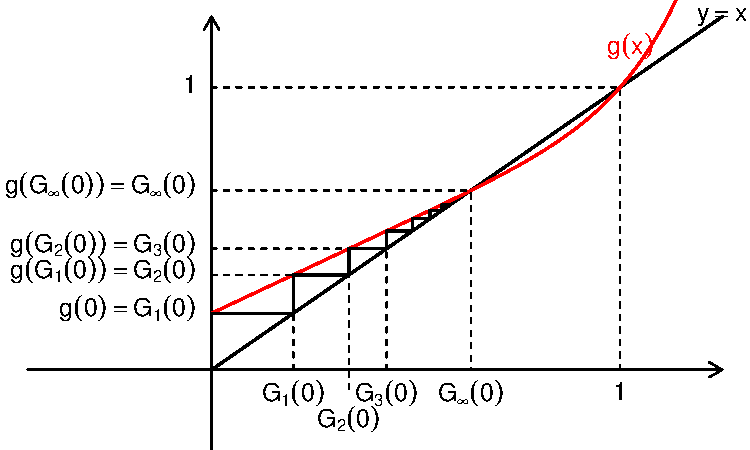
\includegraphics[width=\textwidth]{extinction.pdf}
\end{center}
\end{frame}
% ----------------------------------------------------------------------
\begin{frame}{Formal Proof}
Let $h(s)=g(s)-s$. Observe that
\begin{align*}
h(0)&=g(0)=P_0> 0\\
h'(0)&=g'(0)-1=P_1-1<0\\
\text{Then }\mu > 1
&\Rightarrow h'(1)=\mu-1>0\\
&\Rightarrow h(s)\text{ is increasing near 1}\\
&\Rightarrow h(1-\delta)<h(1)=0\text{ for $\delta>0$ small enough}
\end{align*}
Since $h(s)$ is continuous in $[0,1)$, there must be a root to $h(s)=s$.
The root is unique since
$$
h''(s)=g''(s)=\Sum_{j=2}^{\infty}j(j-1)P_js^{j-2}\ge 0\quad\text{for }0\le s < 1
$$
$h(s)$ is convex in [0,1).
\end{frame}


\begin{frame}{4.5.3 Random Walk w/ Reflective Boundary at 0}
\begin{itemize}
\item State Space $=\{0,1,2,\ldots\}$
\item $P_{01}=1, P_{i,i+1}=p, \;P_{i,i-1}=1-p=q,\;\text{for } i=1,2,3\ldots$
\item Only one class, irreducible
\item For $i<j$, define
\begin{align*}
N_{ij}&=\min\{m> 0: X_m=j|X_0=i\}\\
&=\text{time to reach state $j$ starting in state $i$}
\end{align*}
\item Observe that $N_{0n}=N_{01}+N_{12}+\ldots+N_{n-1,n}$\\
By the Markov property, $N_{01}$, $N_{12},\ldots,N_{n-1,n}$ are indep.
\item Given $X_0=i$
\begin{equation}\label{eq:T1TT}
N_{i,i+1}=
\begin{cases}
1 & \text{if } X_1=i+1\\
1 + N^{*}_{i-1,i}+ N^{*}_{i,i+1} &\text{if } X_1=i-1
\end{cases}
\end{equation}
where $N^{*}_{i-1,i}\sim N_{i-1,i}$, $N^{*}_{i,i+1}\sim N_{i,i+1}$, and $N^{*}_{i-1,i}$, $N^{*}_{i,i+1}$ are indep.
\end{itemize}
\end{frame}
% ----------------------------------------------------------------------
\begin{frame}{Generating Function of $N_{i,i+1}$}
Let $G_{i}(s)$ be the generating function of $N_{i,i+1}$. From \eqref{eq:T1TT},
and by the independence of $N^{*}_{i-1,i}$ and $N^{*}_{i,i+1}$, we get that
$$
G_{i}(s)=ps+q \E[s^{1 + N^{*}_{i-1,i}+ N^{*}_{i,i+1}}]=ps+qsG_{i-1}(s)G_{i}(s)
$$
So
\begin{equation}\label{eq:GiGi-1}
G_i(s)=\frac{ps}{1-qsG_{i-1}(s)}
\end{equation}
Since $N_{01}$ is always 1, we have $G_0(s)=s$. Using the iterative relation \eqref{eq:GiGi-1}, we can find
$$
G_1(s) = \frac{ps}{1-qsG_0(s)}=\frac{ps}{1-qs^2}=ps\sum_{k=0}^{\infty}(qs^2)^k=\sum_{k=0}^{\infty}pq^ks^{2k+1}
$$
So
$\displaystyle
\p(N_{12}=n)
=\begin{cases}
pq^k & \text{if $n=2k+1$ for } k=0,1,2\ldots\\
0    & \text{if $n$ is even}
\end{cases}
$
\end{frame}
% ----------------------------------------------------------------------
\begin{frame}
Similarly,
\begin{align*}
G_2(s) &= \frac{ps}{1-qsG_1(s)}=\frac{ps(1-qs^2)}{1-q(1+p)s^2}\\
&=\frac{ps}{1-q(1+p)s^2}-\frac{pqs^3}{1-q(1+p)s^2}\\
&=ps\Sum_{k=0}^{\infty}(q(1+p)s^2)^k-pqs^3\Sum_{k=0}^{\infty}(q(1+p)s^2)^k\\
&=\Sum_{k=0}^{\infty}pq^k(1+p)^ks^{2k+1}-\Sum_{k=0}^{\infty}pq^{k+1}(1+p)^ks^{2k+3}\\
&=ps+ \Sum_{k=1}^{\infty}pq^k[(1+p)^{k}-(1+p)^{k-1}]s^{2k+1}\\
&=ps+ \Sum_{k=1}^{\infty}p^2q^k(1+p)^{k-1}s^{2k+1}
\end{align*}
So
$$
\p(N_{23}=n)
=\begin{cases}
p    & \text{if }n=1\\
p^2q^k(1\!+\!p)^{k-1} & \text{if $n=2k+1$ for } k=1,2,\ldots\\
0    & \text{if $n$ is even}
\end{cases}
$$
\end{frame}
% ----------------------------------------------------------------------
\begin{frame}{Mean of $N_{i,i+1}$}
Recall that $G'_i(1)=E(N_{i,i+1})$. Let $m_i=E(N_{i,i+1})=G'_i(1)$.
\begin{align*}
G'_i(s)&=\frac{p(1-qsG_{i-1}(s))+ps(qG_{i-1}(s)+qsG'_{i-1}(s))}{(1-qsG_{i-1}(s))^2}\\
&=\frac{p+pqs^2G'_{i-1}(s)}{(1-qsG_{i-1}(s))^2}
\end{align*}
Since $N_{i,i+1}<\infty$, $G_i(1)=1$ for all $i=0,1,\ldots,n-1$.
We have
\[
m_i=G'_i(1)=\frac{p+pqG'_{i-1}(1)}{(1-q)^2}=\frac{1+qG'_{i-1}(1)}{p}=\frac{1}{p}+\frac{q}{p} m_{i-1}
\]
We get the same iterative equation as in Lecture 7.

\end{frame}

\end{document} 